% Options for packages loaded elsewhere
\PassOptionsToPackage{unicode}{hyperref}
\PassOptionsToPackage{hyphens}{url}
%
\documentclass[
]{article}
\usepackage{amsmath,amssymb}
\usepackage{lmodern}
\usepackage{ifxetex,ifluatex}
\ifnum 0\ifxetex 1\fi\ifluatex 1\fi=0 % if pdftex
  \usepackage[T1]{fontenc}
  \usepackage[utf8]{inputenc}
  \usepackage{textcomp} % provide euro and other symbols
\else % if luatex or xetex
  \usepackage{unicode-math}
  \defaultfontfeatures{Scale=MatchLowercase}
  \defaultfontfeatures[\rmfamily]{Ligatures=TeX,Scale=1}
\fi
% Use upquote if available, for straight quotes in verbatim environments
\IfFileExists{upquote.sty}{\usepackage{upquote}}{}
\IfFileExists{microtype.sty}{% use microtype if available
  \usepackage[]{microtype}
  \UseMicrotypeSet[protrusion]{basicmath} % disable protrusion for tt fonts
}{}
\makeatletter
\@ifundefined{KOMAClassName}{% if non-KOMA class
  \IfFileExists{parskip.sty}{%
    \usepackage{parskip}
  }{% else
    \setlength{\parindent}{0pt}
    \setlength{\parskip}{6pt plus 2pt minus 1pt}}
}{% if KOMA class
  \KOMAoptions{parskip=half}}
\makeatother
\usepackage{xcolor}
\IfFileExists{xurl.sty}{\usepackage{xurl}}{} % add URL line breaks if available
\IfFileExists{bookmark.sty}{\usepackage{bookmark}}{\usepackage{hyperref}}
\hypersetup{
  pdftitle={Understanding The Fundamentals Of Hotel Bookings},
  hidelinks,
  pdfcreator={LaTeX via pandoc}}
\urlstyle{same} % disable monospaced font for URLs
\usepackage[margin=1in]{geometry}
\usepackage{graphicx}
\makeatletter
\def\maxwidth{\ifdim\Gin@nat@width>\linewidth\linewidth\else\Gin@nat@width\fi}
\def\maxheight{\ifdim\Gin@nat@height>\textheight\textheight\else\Gin@nat@height\fi}
\makeatother
% Scale images if necessary, so that they will not overflow the page
% margins by default, and it is still possible to overwrite the defaults
% using explicit options in \includegraphics[width, height, ...]{}
\setkeys{Gin}{width=\maxwidth,height=\maxheight,keepaspectratio}
% Set default figure placement to htbp
\makeatletter
\def\fps@figure{htbp}
\makeatother
\setlength{\emergencystretch}{3em} % prevent overfull lines
\providecommand{\tightlist}{%
  \setlength{\itemsep}{0pt}\setlength{\parskip}{0pt}}
\setcounter{secnumdepth}{-\maxdimen} % remove section numbering
\ifluatex
  \usepackage{selnolig}  % disable illegal ligatures
\fi

\title{Understanding The Fundamentals Of Hotel Bookings}
\author{true}
\date{08-27-2021}

\begin{document}
\maketitle

\textbf{Introduction}

\emph{Travel holds one of the biggest annual expenses in the USA.
According to the US Travel Association in the year 2019 alone,total
international and domestic traveler spending generated \$2.6 trillion in
economic output, measuring up to 2.9 percent of the nations gross
domestic product(GDP) and most importantly generated over 15.8 million
jobs in the country.}

\emph{Today, with the constant development of technology and online
services, the traveling industry has become more accessible and
affordable to everyone. The statistical portal has shown that around
eighty eight percent of Americans prefer to book or have booked their
hotel online using the internet portals (2017).Online booking travel
agents, travel websites and advanced systems have immensely affected the
direct relationship of the hotel management and guests.While there are
certain advantages and disadvantages of hotel booking online or offline
using travel agents, the statistics of avid travelers in the USA shows
that competition is high when it comes to finding the perfect deal for
stay. Additionally, online booking has been said to guarantee customers
to get the lowest price possible, there have been issues of lack of
transparency and chances of canceling/ moving dates last minute which we
will also be analyzing the data for today.}

\emph{Studies have shown that established companies benefit and save a
large amount of revenue when they are dealing with repeated customers as
they do not have to have additional advertisement expenses and repeated
customers can also reflect the success of a company. We will be
analyzing and plotting graphs on repeated customers according to each
year (2015-2017) as well as determining which of the months do customers
prefer to travel back.}

\textbf{Research Question}

\emph{For this project my research questions would be focused on three
major categories in order to identify the optimal time for traveling.
What is the best time of the year to book hotels? Out of the resort
hotel and city hotels, which hotel recieve higher number of customers?
What is the most popular source of travel agents (online or offline TA).
I am personally interested in this topic as I enjoy traveling myself,
especially after the COVID-19 pandemic, the travel industry has
struggled to keep their doors open. Now with the prevalence of
vaccinations and proper covid guidelines, the traveling industry is
expected to grow drastically.} \emph{In this paper, we will also be
discussing the peak times of the year where it is a good idea to travel
and book for hotels, it can be a struggle for many people to travel
during times where locations are packed with customers. We will also
identify the most popular source of booking trips and determining if it
is through online services such as tripadvisor, travelhelp and expedia
without any direct connection to the hotel or through offline travel
agents that connect with customers directly.}

\textbf{Data Selection}

\emph{The data set we are analyzing is a single file which aims to
compare various booking information between two hotels, specifically a
city hotel and a resort hotel. The data consists of 32 columns through
which I have worked to determine the above mentioned research
questions.}

\textbf{Load the packages} \emph{In order to look at the data we will be
loading some packages such as tidyverse,dbplyr, ggplot2, stringi,
rmarkdown)}

\begin{verbatim}
## -- Attaching packages --------------------------------------- tidyverse 1.3.1 --
\end{verbatim}

\begin{verbatim}
## v ggplot2 3.3.3     v purrr   0.3.4
## v tibble  3.1.2     v dplyr   1.0.7
## v tidyr   1.1.3     v stringr 1.4.0
## v readr   1.4.0     v forcats 0.5.1
\end{verbatim}

\begin{verbatim}
## -- Conflicts ------------------------------------------ tidyverse_conflicts() --
## x dplyr::filter() masks stats::filter()
## x dplyr::lag()    masks stats::lag()
\end{verbatim}

\begin{verbatim}
## 
## Attaching package: 'dbplyr'
\end{verbatim}

\begin{verbatim}
## The following objects are masked from 'package:dplyr':
## 
##     ident, sql
\end{verbatim}

\textbf{Read in the database}

\emph{One of the most important step to start with would be reading in
the database. We will be working with the hotel\_booking database. The
data is a single file which has information to compare various booking
information between two hotels, specifically a city hotel and a resort
hotel. The data consists of 32 columns through which I have selected
five variables to research the above mentioned questions}

\emph{As you can see I have named my database ``book''}

\begin{verbatim}
## 
## -- Column specification --------------------------------------------------------
## cols(
##   .default = col_double(),
##   hotel = col_character(),
##   arrival_date_month = col_character(),
##   meal = col_character(),
##   country = col_character(),
##   market_segment = col_character(),
##   distribution_channel = col_character(),
##   reserved_room_type = col_character(),
##   assigned_room_type = col_character(),
##   deposit_type = col_character(),
##   agent = col_character(),
##   company = col_character(),
##   customer_type = col_character(),
##   reservation_status = col_character(),
##   reservation_status_date = col_date(format = "")
## )
## i Use `spec()` for the full column specifications.
\end{verbatim}

\begin{verbatim}
## [1] 119390     32
\end{verbatim}

\emph{Next step would be using the dim() function, it allows us to
retrieve or set the dimensions of an object in R.For our current
database ``book'' it is determined to have 32 columns and 119390 rows.}

\begin{verbatim}
##  [1] "hotel"                          "is_canceled"                   
##  [3] "lead_time"                      "arrival_date_year"             
##  [5] "arrival_date_month"             "arrival_date_week_number"      
##  [7] "arrival_date_day_of_month"      "stays_in_weekend_nights"       
##  [9] "stays_in_week_nights"           "adults"                        
## [11] "children"                       "babies"                        
## [13] "meal"                           "country"                       
## [15] "market_segment"                 "distribution_channel"          
## [17] "is_repeated_guest"              "previous_cancellations"        
## [19] "previous_bookings_not_canceled" "reserved_room_type"            
## [21] "assigned_room_type"             "booking_changes"               
## [23] "deposit_type"                   "agent"                         
## [25] "company"                        "days_in_waiting_list"          
## [27] "customer_type"                  "adr"                           
## [29] "required_car_parking_spaces"    "total_of_special_requests"     
## [31] "reservation_status"             "reservation_status_date"
\end{verbatim}

\emph{After determining that we have 32 columns, the colnames()
functions helps us look at the titles for each of the variables we have
data for}

\textbf{The five variables we will be looking at in this paper are}
\emph{1. Hotel} \emph{2. Date of Arrival(Year)} \emph{3. Date of
Arrival(Month)} \emph{4. Repeated Guest} \emph{5. Market Segment}

\textbf{In order to separate and piping selected variables I am using
the package dplyr and using the select() function as seen below, our new
file will be called ``d''}

\begin{verbatim}
## # A tibble: 119,390 x 5
##    hotel     arrival_date_year arrival_date_mon~ is_repeated_gue~ market_segment
##    <chr>                 <dbl> <chr>                        <dbl> <chr>         
##  1 Resort H~              2015 July                             0 Direct        
##  2 Resort H~              2015 July                             0 Direct        
##  3 Resort H~              2015 July                             0 Direct        
##  4 Resort H~              2015 July                             0 Corporate     
##  5 Resort H~              2015 July                             0 Online TA     
##  6 Resort H~              2015 July                             0 Online TA     
##  7 Resort H~              2015 July                             0 Direct        
##  8 Resort H~              2015 July                             0 Direct        
##  9 Resort H~              2015 July                             0 Online TA     
## 10 Resort H~              2015 July                             0 Offline TA/TO 
## # ... with 119,380 more rows
\end{verbatim}

\emph{Next, lets clean our data for easier analysis using the unique
function. Unique functions will return our data frame after removing
duplicate elements/rows.We will apply this function to each of our
variable}

\begin{verbatim}
## [1] 2015 2016 2017
\end{verbatim}

\begin{verbatim}
##  [1] "July"      "August"    "September" "October"   "November"  "December" 
##  [7] "January"   "February"  "March"     "April"     "May"       "June"
\end{verbatim}

\begin{verbatim}
## [1] "Resort Hotel" "City Hotel"
\end{verbatim}

\begin{verbatim}
## [1] 0 1
\end{verbatim}

\begin{verbatim}
## [1] "Direct"        "Corporate"     "Online TA"     "Offline TA/TO"
## [5] "Complementary" "Groups"        "Undefined"     "Aviation"
\end{verbatim}

\textbf{\emph{DATA VISUALIZATION}}

\emph{Count of repeated hotel}

\begin{verbatim}
## # A tibble: 2 x 2
##   hotel            n
##   <chr>        <int>
## 1 City Hotel   79330
## 2 Resort Hotel 40060
\end{verbatim}

\emph{Count of repeated year}

\begin{verbatim}
## # A tibble: 3 x 2
##   arrival_date_year     n
##               <dbl> <int>
## 1              2015 21996
## 2              2016 56707
## 3              2017 40687
\end{verbatim}

\emph{Count of arrival\_date\_month}

\begin{verbatim}
## # A tibble: 12 x 2
##    arrival_date_month     n
##    <chr>              <int>
##  1 April              11089
##  2 August             13877
##  3 December            6780
##  4 February            8068
##  5 January             5929
##  6 July               12661
##  7 June               10939
##  8 March               9794
##  9 May                11791
## 10 November            6794
## 11 October            11160
## 12 September          10508
\end{verbatim}

\emph{Count of market\_segment}

\begin{verbatim}
## # A tibble: 8 x 2
##   market_segment     n
##   <chr>          <int>
## 1 Aviation         237
## 2 Complementary    743
## 3 Corporate       5295
## 4 Direct         12606
## 5 Groups         19811
## 6 Offline TA/TO  24219
## 7 Online TA      56477
## 8 Undefined          2
\end{verbatim}

\emph{Count of repeated guest}

\begin{verbatim}
## # A tibble: 2 x 2
##   is_repeated_guest      n
##               <dbl>  <int>
## 1                 0 115580
## 2                 1   3810
\end{verbatim}

\emph{Using the count() function, let us asses the number of variables
and count of each subset of variable. This will give us an exact number
of data in each category}

\emph{From this graph, we can determine the highest number of travelers
in 2016 and lowest in 2015}
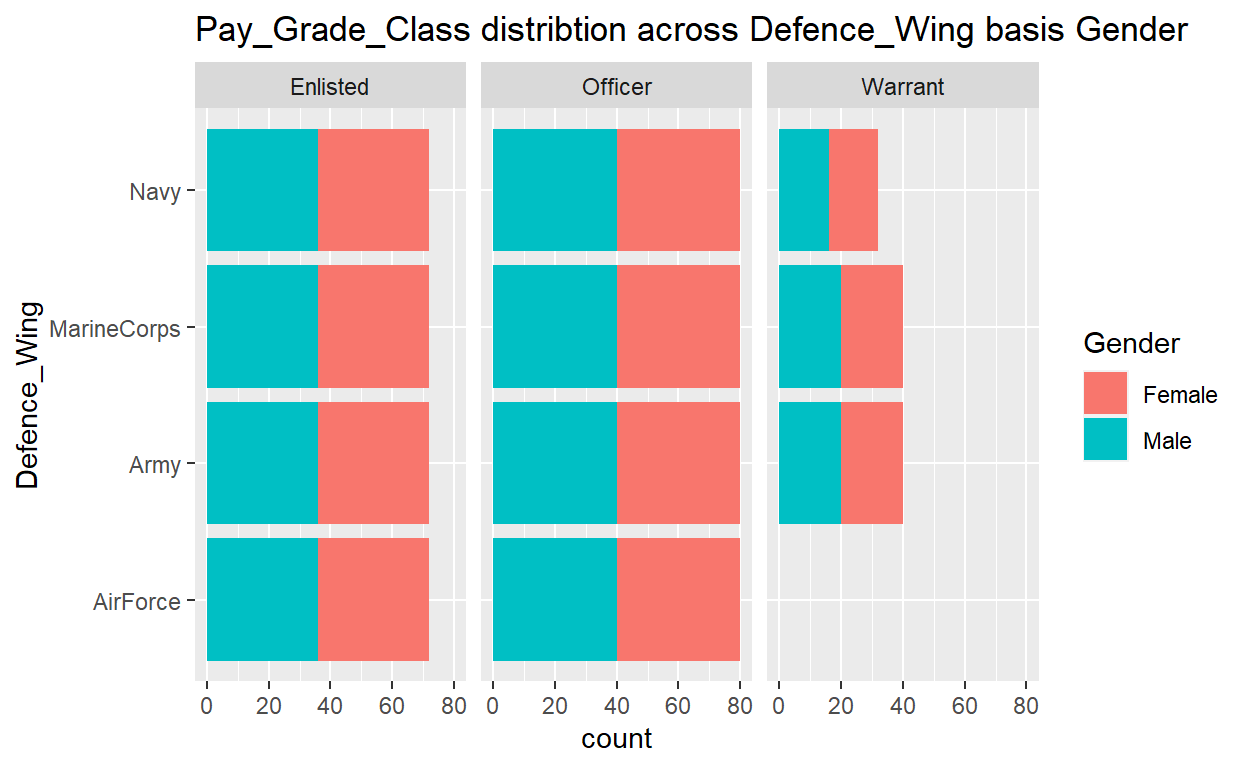
\includegraphics{finalprojectzutima_files/figure-latex/unnamed-chunk-13-1.pdf}
\textbf{Arrival Date Year}

\emph{The bar shows the number of guests that booked hotels each month
from 2015-2017 at the particular hotels. We can see from the graph there
were highest number of bookings in August and lowest number of bookings
in January.}
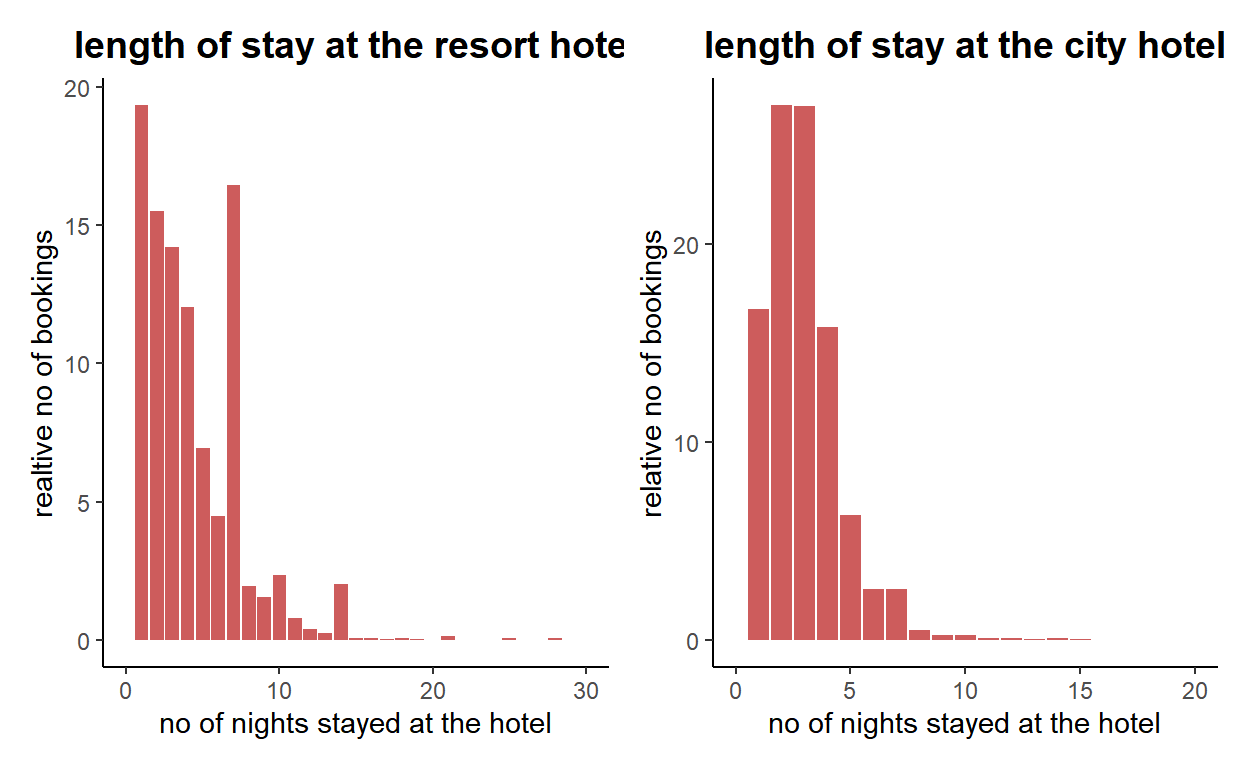
\includegraphics{finalprojectzutima_files/figure-latex/unnamed-chunk-14-1.pdf}
\textbf{Preference in Month}

\emph{From this graph, we can see that guests overall preferred the City
Hotel over Resort}
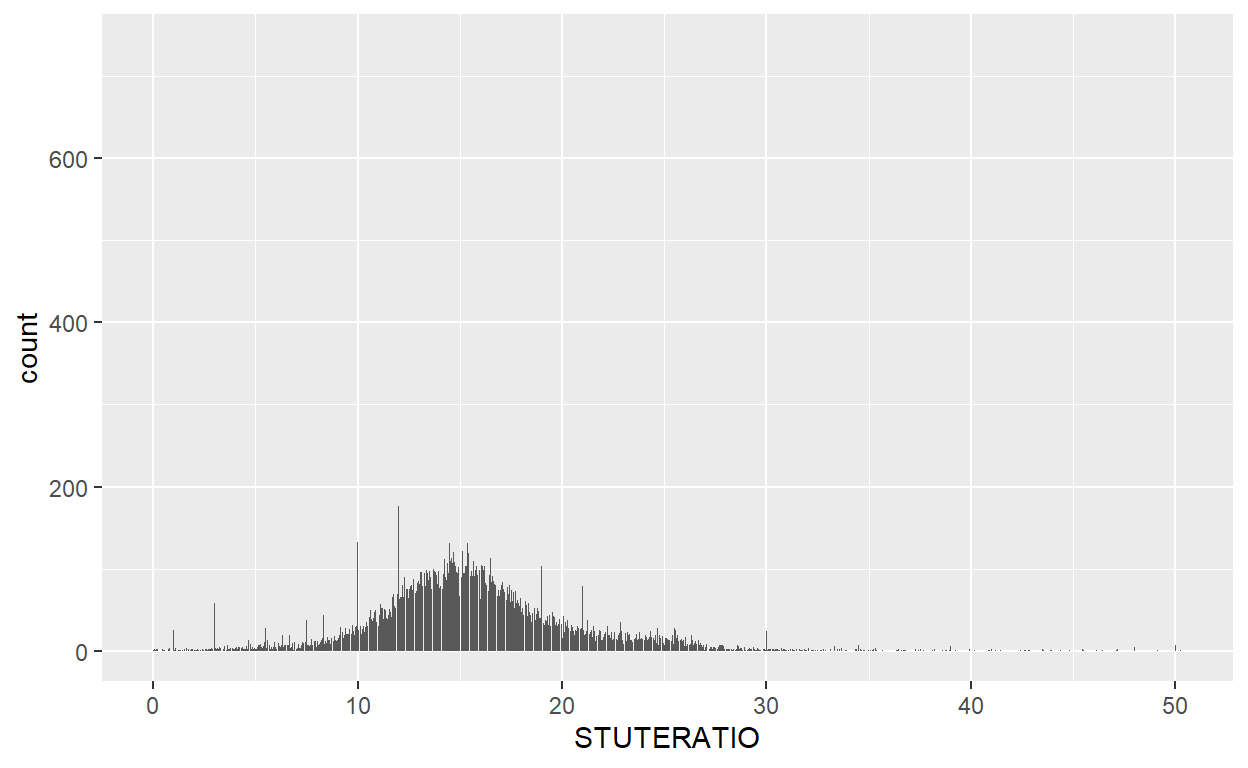
\includegraphics{finalprojectzutima_files/figure-latex/unnamed-chunk-15-1.pdf}
\textbf{Preference in Hotel} \textbf{Filter Database}

\textbf{Arrange Database}

\begin{verbatim}
## # A tibble: 6 x 3
## # Groups:   hotel, arrival_date_year [6]
##   hotel        arrival_date_year     n
##   <chr>                    <dbl> <int>
## 1 City Hotel                2015 13682
## 2 City Hotel                2016 38140
## 3 City Hotel                2017 27508
## 4 Resort Hotel              2015  8314
## 5 Resort Hotel              2016 18567
## 6 Resort Hotel              2017 13179
\end{verbatim}

\begin{verbatim}
## Warning: Ignoring unknown parameters: binwidth, bins, pad
\end{verbatim}

\includegraphics{finalprojectzutima_files/figure-latex/arrange-1.pdf}
\includegraphics{finalprojectzutima_files/figure-latex/arrange-2.pdf}

\begin{verbatim}
## # A tibble: 4 x 3
## # Groups:   hotel, is_repeated_guest [4]
##   hotel        is_repeated_guest     n
##   <chr>                    <dbl> <int>
## 1 City Hotel                   0 77298
## 2 City Hotel                   1  2032
## 3 Resort Hotel                 0 38282
## 4 Resort Hotel                 1  1778
\end{verbatim}

\begin{verbatim}
## Warning: Ignoring unknown parameters: binwidth, bins, pad
\end{verbatim}

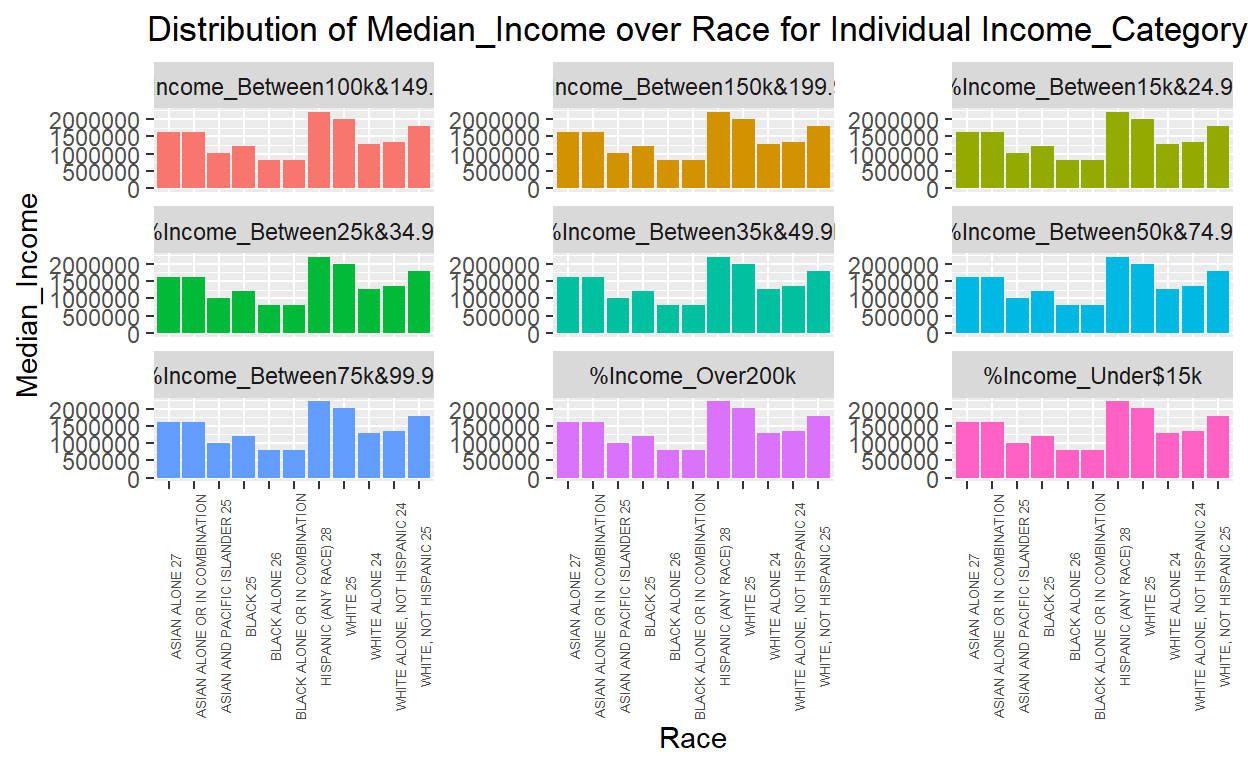
\includegraphics{finalprojectzutima_files/figure-latex/unnamed-chunk-16-1.pdf}

\begin{verbatim}
## # A tibble: 6 x 3
## # Groups:   arrival_date_year, is_repeated_guest [6]
##   arrival_date_year is_repeated_guest     n
##               <dbl>             <dbl> <int>
## 1              2015                 0 21355
## 2              2015                 1   641
## 3              2016                 0 54929
## 4              2016                 1  1778
## 5              2017                 0 39296
## 6              2017                 1  1391
\end{verbatim}

\begin{verbatim}
## Warning: Ignoring unknown parameters: binwidth, bins, pad
\end{verbatim}

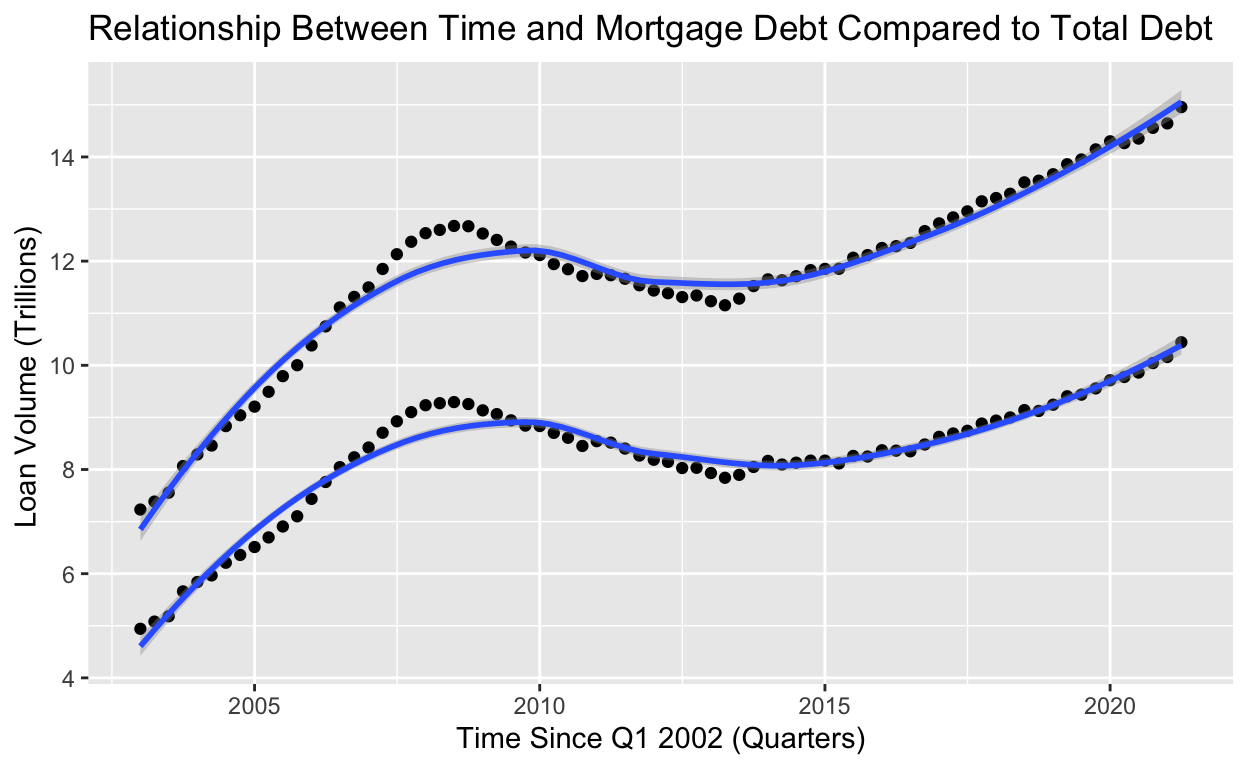
\includegraphics{finalprojectzutima_files/figure-latex/unnamed-chunk-17-1.pdf}
*The graph shows the number of repeated guests in each city hotel and
resort hotel, you can also see in the number of repeated guests each
year.

\begin{verbatim}
## # A tibble: 26 x 3
## # Groups:   arrival_date_year, arrival_date_month [26]
##    arrival_date_year arrival_date_month     n
##                <dbl> <chr>              <int>
##  1              2015 August              3889
##  2              2015 December            2920
##  3              2015 July                2776
##  4              2015 November            2340
##  5              2015 October             4957
##  6              2015 September           5114
##  7              2016 April               5428
##  8              2016 August              5063
##  9              2016 December            3860
## 10              2016 February            3891
## # ... with 16 more rows
\end{verbatim}

\begin{verbatim}
## Warning: Ignoring unknown parameters: fill
\end{verbatim}

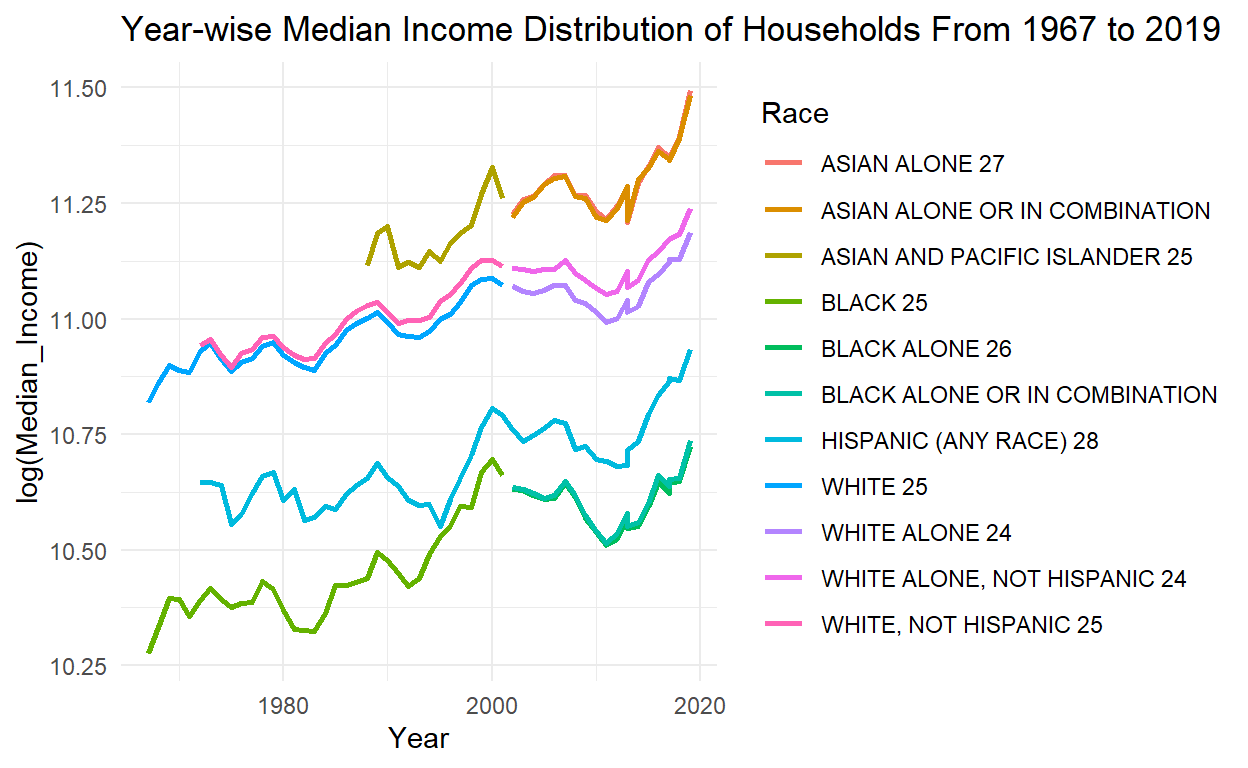
\includegraphics{finalprojectzutima_files/figure-latex/unnamed-chunk-18-1.pdf}

\emph{Organizing the database according to year and month using the
geom\_histogram()}

\begin{verbatim}
## Warning: Ignoring unknown parameters: binwidth, bins, pad
\end{verbatim}

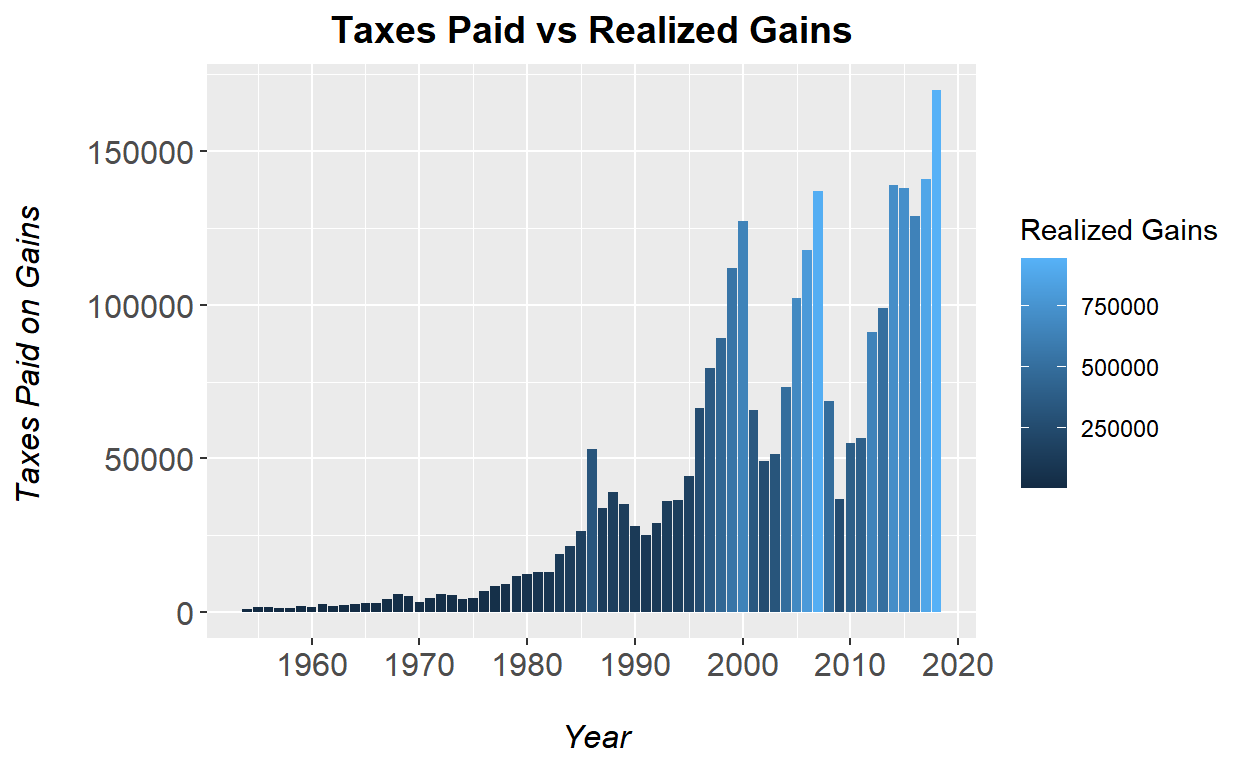
\includegraphics{finalprojectzutima_files/figure-latex/unnamed-chunk-19-1.pdf}

\textbf{Reflection}

\emph{This project was my initial introduction to R and rstudio
projects, therefore when I was working through understanding the
concepts there were some roadblocks. However, the data set that I had
selected ``hotel\_bookings'' was a fairly advanced and straightforward
dataset. It helped to complete this assignment in chunks spread out
through the three weeks as I was able to identify my issues easily and
work accordingly. The initial difficulty I had with the paper was in
github as I was not able to identify my directory and connect it to the
main repository. This created an error in R where the most important
section ``Read in Data'' was not running. Without establishing this
connection further analysis was not possible. I learned that in order to
have your data in the code we have to establish the connection by piping
the data to the necessary assigned folders. Once I was able to code the
connection the error was removed}

\begin{itemize}
\tightlist
\item
\end{itemize}

\textbf{Conclusion}

\emph{This conclusion aims to answer the three major categories of
research questions I had identified. Lets us look at them in order. For
the first question asking the best time of the year to book hotels, the
data shows that between the year of 2015-2017. The total number of
guests in 2015, 2016 and 2017 were 21996,56707 and 40687 accordingly.The
most popular month in 2015 is in September guests = 5114 and least
popular month in 2015 is in November guests = 2340. If we further look
at the data we can see that the most popular month in 2016 was was
during the month of October guest = 6203 and lowest in 2016 was in the
month of January guests = 2248.Although, more research is required, we
can argue that the most busiest time in the year is August-October and
least busiest is January-April.For our second question, overall out of
both the highest guests year and lowest guest year, the city hotel was
able to accumulate and serve the majority of people in comparison as we
can see in our graph as well.The total number of guests were 119390, in
which city hotel guests 79330 and resort guests had 40060, with a
staggering difference of 39270.According to our data we can state that
city hotels receive higher number of customers. It is also interesting
to note that city hotels(2032) also receive higher number of repeated
guests in comparison to resort hotels(1178) Lastly to analyze which is
the most popular and reliable source for booking hotels and arranging
travel plans. From this data and graphs we can determine that similarly
to the statistic we had introduced in the first paragraph that according
to US Travel Association, online travel agents are the most popular and
in demand service among all the other market segment dominating the
offline travel agents. To conclude, understanding the different aspects
of this data will be helpful in organizing future travel plans to
determine the best price, service as well as time of the month. Further
research and data should be collected to improve the relability and
validity}

\textbf{References}

\emph{Hotel Booking Demand (February 2019.)
\url{https://www.kaggle.com/jessemostipak/hotel-booking-demand}}

\emph{Qualitative study of online hotel booking systems (Henry, 2018)
\url{https://pmworldlibrary.net/wp-content/uploads/2018/03/pmwj68-Mar2018-Henry-study-of-online-booking-systems-student-paper.pdf}}

\emph{US Travel Association (2021)
\url{https://www.ustravel.org/answersheet} }

\end{document}
